\chapter{System topology}
\label{cha:SystemTopology}
%利用热力学原理进行定性分析。提炼出创新点。
\section{System topology design}
\label{sec:std}

The objective of this research is to investigate the equipment of solar thermal power generation system, to propose, develop and optimize a cascade solar thermal system depending on the advantages and disadvantages of existing solar thermal power generation technologies. 

Three solar thermal power generation technologies are commercially proven -- parabolic trough, parabolic dish and solar tower. 
Considering the future deployment of solar cascade demo system, two solar thermal technologies, parabolic trough and parabolic dish, are chosen as the basic systems for the design of cascade solar thermal power system. For the cascade utilization of the high temperature heat source obtained from the parabolic dish receiver, air (or nitrogen) is used as the HTF to transfer the heat collected.
Figure~\ref{fig:PTPD} shows the schematic diagrams of a parabolic trough system and a parabolic dish system. To make the system structure diagrams in this thesis more clearly and consistent, legends of the components that may appear in solar power systems are listed in Figure~\ref{fig:Legends}.

\begin{figure}[!ht]
\centering
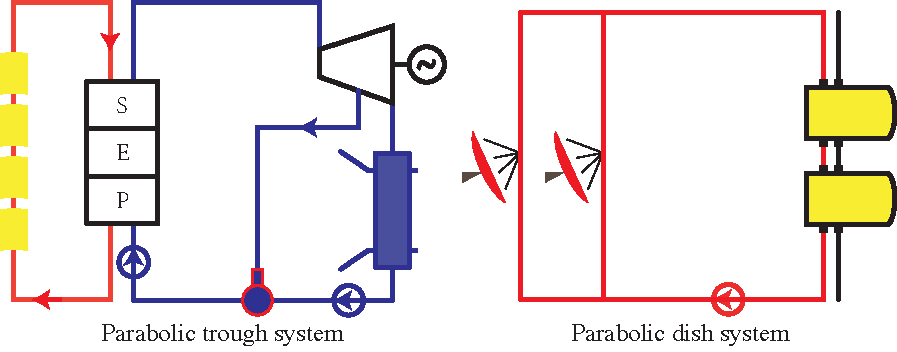
\includegraphics[width=0.8\textwidth]{fig/PTPD.pdf}
\caption{Schematic diagrams of a parabolic trough system and a parabolic dish system}
\label{fig:PTPD}
\end{figure}

\begin{figure}[!ht]
\centering
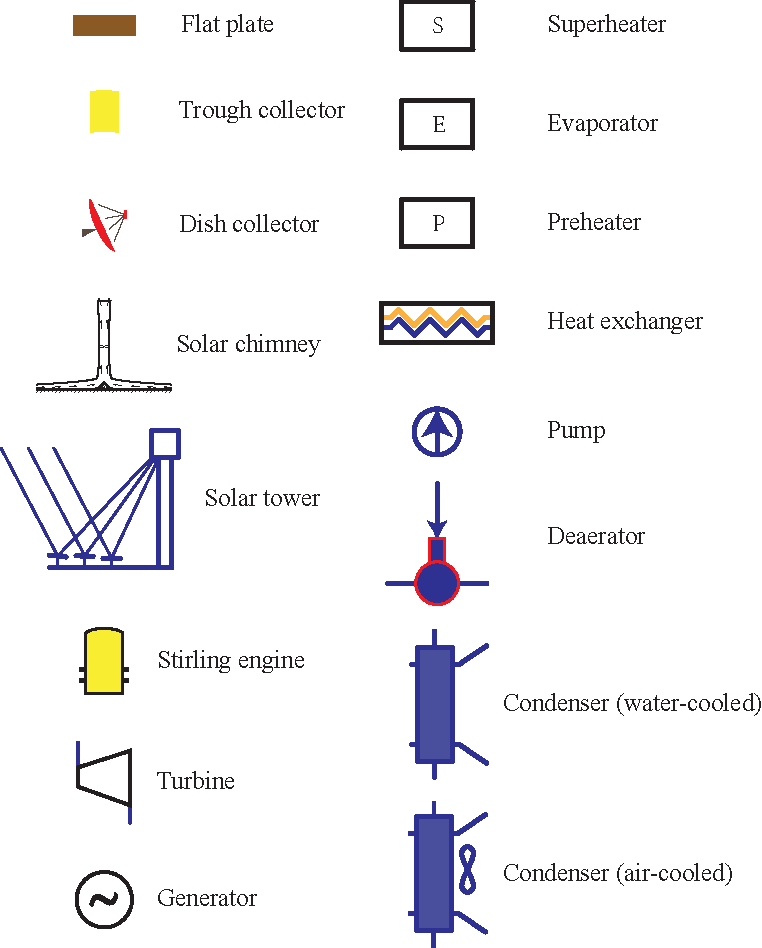
\includegraphics[width=0.8\textwidth]{fig/Legends.pdf}
\caption{Components in solar power systems}
\label{fig:Legends}
\end{figure}

With different considerations (such as water Rankine cycle or ORC, combination of different systems, connection types of collectors, etc) of the cascade system topology, multiple combination topologies may be used for cascade systems. To get the most suitable system topology, these considerations will be analyzed in the following sections. 

\subsection{Rankine cycle fluid}
\label{sec:RankineCycleFluid}

\begin{figure}[!ht]
\centering 
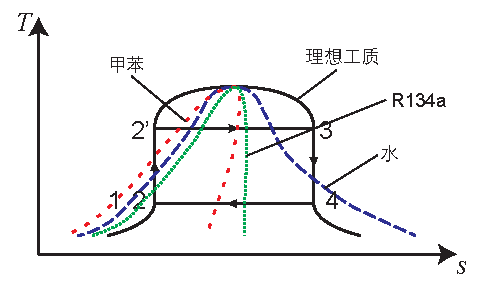
\includegraphics[width=0.5\textwidth]{fig/idealTs}
\caption{Temperature-entropy diagram of an ideal working fluid}\label{fig:idealTs}
\end{figure}

An ideal working fluid would have the temperature-entropy diagram given in Figure~\ref{fig:idealTs}. The following characteristics listed by Abbin and Leuenberger~\cite{Abbin1977} describe this fluid:
\begin{itemize}
  \item The heat capacity of the liquid phase should be small. This makes the curve 22' in Figure~\ref{fig:idealTs} almost vertical.
  \item The critical point should be above the highest operating temperature to allow all heat to be added at that temperature.
  \item The vapor pressure at the highest operating temperature should be moderate for safety reasons and to reduce the cost of the equipment.
  \item The vapor pressure at the condensing temperature should be above atmospheric pressure to prevent air leakage into the system.
  \item The specific volume of the vapor at state 4 should be small to avoid large-diameter turbine wheels, casings, and heat exchangers.
  \item The saturated vapor curve 3-4 in Figure~\ref{fig:idealTs} should be vertical to avoid expansion into the wet vapor region (negative $ds/dT$) or expansion into the superheat region (positive $ds/dT$).
  \item For low-power turbine applications, the fluid should have a high molecular weight to minimize the rotational speed and/or the number of turbine stages and to allow for reasonable mass flow rates and turbine nozzle areas.
  \item The fluid should be liquid at atmospheric pressure and temperature for ease of handling and containment.
  \item The freezing point should be lower than the lowest ambient operating temperature.
  \item The fluid should have good heat-transfer properties, be inexpensive, thermally stable at the highest operating temperature, nonflammable, noncorrosive, nontoxic, and so on.
\end{itemize}

Water is the most commonly used fluid for Rankine cycle, it is more mature to design Rankine cycle components for steam systems than any other liquid. It is inexpensive to use (although boiler-grade water must be highly distilled and thus costs more than tap water), sealing of the high-pressure portions of a Rankine cycle using steam is not critical. Non-flammability and ready availability of steam are additional advantages. Because it has a critical temperature and pressure of 374$\mathrm{^\circ C}$ and 22.1$\mathrm{MPa}$, it can be used for systems operating at fairly high temperatures with most of the heat addition (at constant temperature) and at moderate pressure. Figure~\ref{fig:TypicalSteamRankineSolarSystem} shows the schematic diagram of a typical steam Rankine cycle solar system.

\noindent \begin{figure}[htbp]
\centering
	\begin{subfigure}[b]{0.4\columnwidth}
	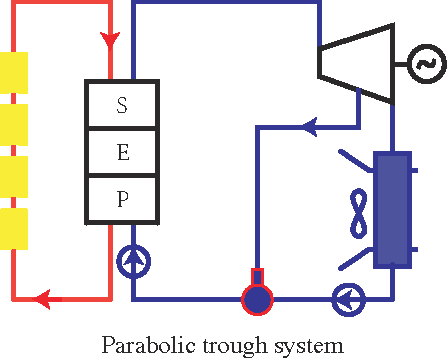
\includegraphics[width = \columnwidth]{fig/TypicalSteamRankineSolarSystem}
	\caption{}\label{fig:TypicalSteamRankineSolarSystem}
	\end{subfigure}
	~
\begin{subfigure}[b]{0.4\columnwidth}
	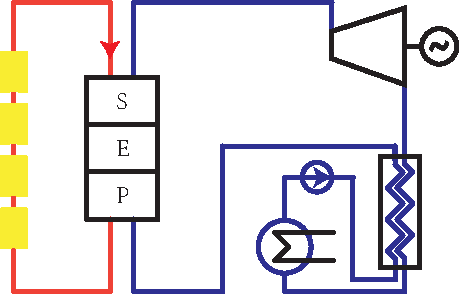
\includegraphics[width = \columnwidth]{fig/TypicalOrganicRankineSolarSystem}
	\caption{}\label{fig:TypicalOrganicRankineSolarSystem}
	\end{subfigure}
	\caption{Schematic diagrams of two types of Rankine cycle solar system}
	\label{fig:TwoTypesOfRankineCycle}
\end{figure}

There are some disadvantages for steam as the Rankine cycle fluid. The low temperature characteristics of steam are not ideal because the steam has a low vapor pressure (see Table~\ref{tab:waterT_P}) and a very low density at ambient temperature. Therefore, sealing air from low pressure components is a major design problem.
\begin{table}[htbp]
	\caption{Saturated steam pressure at the corresponding temperature}
	\begin{center}
	\begin{tabular}{cccccccccc}
		\toprule	
		    $T$(K)    &	373.15	    &    363.15    &    353.15    &    343.15    &    333.15    &    323.15    &    313.15    &    303.15    &    293.15\\
		\midrule	
		    $p$(Pa)    &    101322        &    70117    &    47373    &    31176    &    19932    &    12344    &    7381    &    4246    &    2339\\
		\bottomrule
	\end{tabular}
	\end{center}
	\label{tab:waterT_P}
\end{table}

The organic Rankine cycle can be used in the solar parabolic trough technology in place of the usual steam Rankine cycle. The ORC allows power generation at lower capacities and with a lower collector temperature, and hence the possibility for low-cost, small scale decentralized CSP units. Most organic fluids used in organic Rankine cycle are drying fluids. The vapor leaving the expander still contains heat that can be transferred to the compressed liquid stream because the turbine outlet temperature is above the condenser temperature. A vapor-to-liquid heat exchanger, known as a regenerator, is typically used for this purpose.
Figure~\ref{fig:TypicalOrganicRankineSolarSystem} shows the schematic diagram of a typical organic Rankine cycle solar system. 

%\begin{figure}[!ht]
%\centering 
%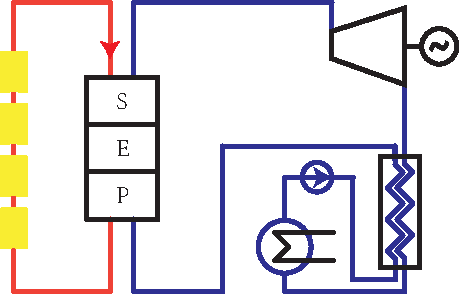
\includegraphics[width=0.7\textwidth]{fig/TypicalOrganicRankineSolarSystem}
%\caption{Schematic diagram of a typical organic Rankine cycle solar system}\label{fig:TypicalOrganicRankineSolarSystem}
%\end{figure}

Compared with steam for the Rankine cycle, it has the following advantages:
\begin{itemize}
  \item  Small turbine head allows for moderate shaft speed and a single- or two-stage design.
    \item Low volume ratio facilitates the flow path design.
    \item High volume flow and low velocity of sound results in reasonable flow areas.
    \item Low temperature drop during expansion reduces thermal stress problems.
    \item Dry expansion avoids blade erosion caused by vapor wetness.
    \item Low system pressure facilitates housing design.
  \end{itemize}

\subsection{Solar chimney}
\label{sec:sc}
Solar chimney, also known as solar updraft tower, directly (without concentration) uses the sun's heat to generate power. It uses solar radiation to increase the internal air temperature to form a flow to the chimney located at the middle of the roof. Figure~\ref{fig:SolarChimney} shows the schematic diagram of a typical solar chimney power plant. In this plant, air is heated by the green house effect under the translucent roof. As the roof is open at its periphery, air flows into the plant due to different density distribution. Hot air flows into the chimney because of buoyancy. An electricity-generating turbine is set in the path of the air current to convert the kinetic energy of the flowing air into electricity.

\begin{figure}[!ht]
\centering 
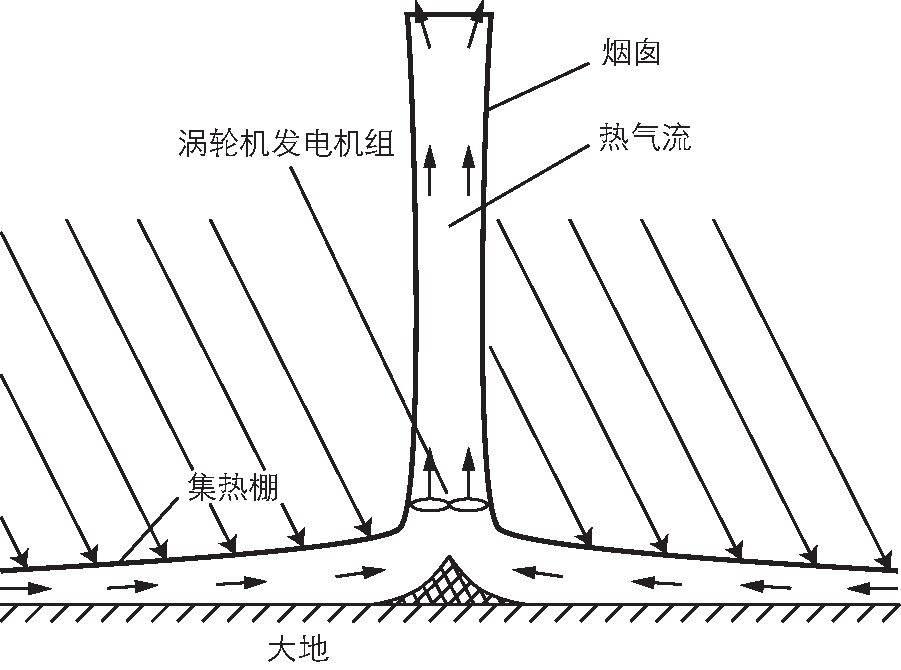
\includegraphics[width=0.5\textwidth]{fig/SolarChimney}
\caption{Schematic diagram of a solar chimney power plant}\label{fig:SolarChimney}
\end{figure}

The solar chimney can use the low temperature (low grade energy) for power generation. So the combination of parabolic trough system and solar chimney is considered an effective way for energy cascade utilization. In the combined system, the condenser in the Rankine cycle is air cooled. The fan blows the hot air that has cooled the condenser into the solar chimney power plant from its periphery. The hot air stream converges at the bottom of chimney, flows upward with the action of buoyancy and drives the turbine in the chimney.
Energy of the hot air can be utilized by the solar chimney. Figure~\ref{fig:CombinedSolarChimney} shows an example of the combined system. 

\begin{figure}[!ht]
\centering 
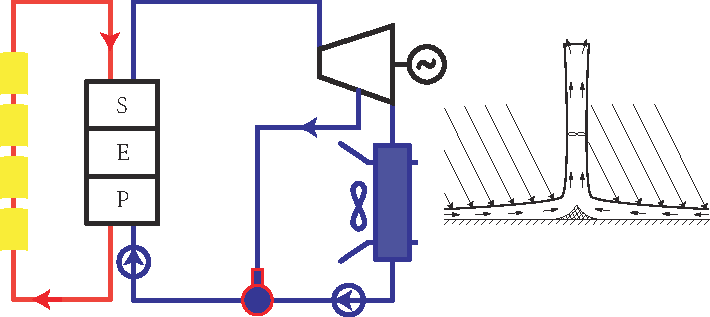
\includegraphics[width=0.7\textwidth]{fig/CombinedSolarChimney}
\caption{Schematic diagram of a combined solar trough and chimney power system}\label{fig:CombinedSolarChimney}
\end{figure}

\subsection{Collector series connection}
\label{sec:csc}

Considering different heat collecting temperatures of different types of collectors, series connection of different types of collectors can be a feasible choice for solar cascade collection. Trough collectors and Fresnel collectors have better performance and lower cost for lower temperature heat collection. Dish collectors and solar towers are more suitable for higher temperature heat collection. Serial connection utilize the advantages of different types of collectors. Figure~\ref{fig:SeriesCollector} shows an example of a cascade system using collector series connection. In this system, air, the HTF, is preheated by parabolic collectors before it flows into the parabolic dish collectors.

\begin{figure}[!ht]
\centering 
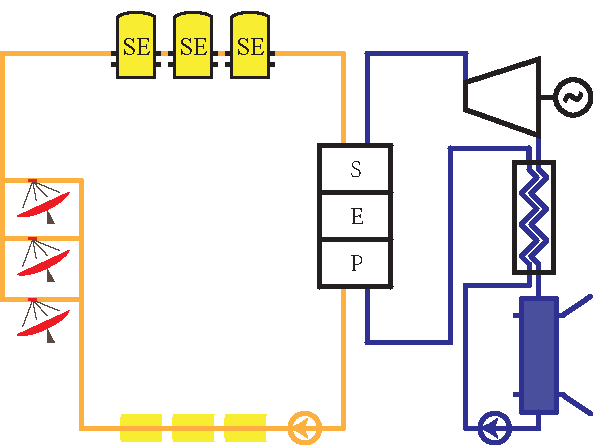
\includegraphics[width=0.5\textwidth]{fig/SeriesCollector}
\caption{Schematic diagram of a cascade system using collector series connection}\label{fig:SeriesCollector}
\end{figure}

\subsection{Direct steam generation}

Direct steam generation (DSG) in parabolic troughs is considered as an attractive option for both economic and efficiency improvement of for solar thermal electricity generation applications.~\cite{Montes2011,Elsafi2015} It allows higher cycle temperatures and, consequently, higher Rankine cycle efficiencies.~\cite{Fraidenraich2013} In conventional parabolic trough solar plants, HTF (typically synthetic oil or melton salt) is used in the solar field. It leads to high pressure drop, limits the HTF related equipment operation, maintenance and cost. Besides, the highest temperature of the Rankine cycle is limited by the HTF temperature, and large temperature difference exists between the HTF and working fluid of the Rankine cycle. So generating steam in the receiver tubes (direct steam generation, DSG) of the solar collector is one of the directions to reduce the cost and increase the efficiency of the PTC systems. Figure~\ref{fig:DSG} shows the schematic diagram of a typical DSG solar system.

\begin{figure}[!ht]
\centering 
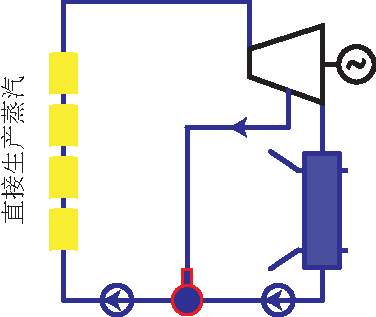
\includegraphics[width=0.5\textwidth]{fig/DSG}
\caption{schematic diagram of a typical solar trough using DSG}\label{fig:DSG}
\end{figure}

\subsection{Heat exchanger between circuits}
\label{sec:hebc}

Heat transfer between different circuits can be applied for cascade utilization of the heat collected. Depending on the two basic solar system in~\ref{fig:PTPD}, there are two types of heat exchangers that can be applied in the solar system.

In the first type, air-oil heat exchanger is applied to transfer heat between the air circuit and the oil circuit. Figure~\ref{fig:air-oil} shows an example of solar system using this type of heat exchanger. In this system, after providing heat for the Stirling engines, the hot air flows through the air-oil heat exchanger and provides heat for the oil. 

\begin{figure}[h]
\centering 
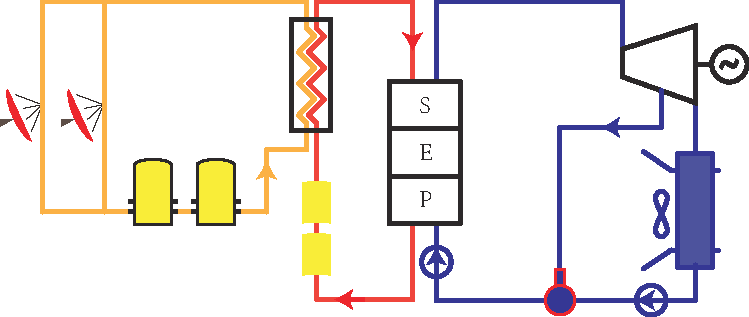
\includegraphics[width=0.7\textwidth]{fig/air-oil}
\caption{Schematic diagram of a solar system using air-oil heat exchanger}\label{fig:air-oil}
\end{figure}

In the second type, air-water heat exchanger is applied to transfer heat between the air circuit and the water circuit. Figure~\ref{fig:air-water_1} and Figure~\ref{fig:air-water_2} show two different kinds of solar systems using this type of heat exchanger. In Figure~\ref{fig:air-water_1}, after providing heat for the Stirling engines, the hot air flows through the air-water heat exchanger and provides heat for superheating. In Figure~\ref{fig:air-water_2}, after providing heat for the Stirling engines, the hot air flows through the air-water heat exchanger and provides heat for preheating. 

\noindent \begin{figure}[htbp]
\centering
	\begin{subfigure}[b]{0.4\columnwidth}
	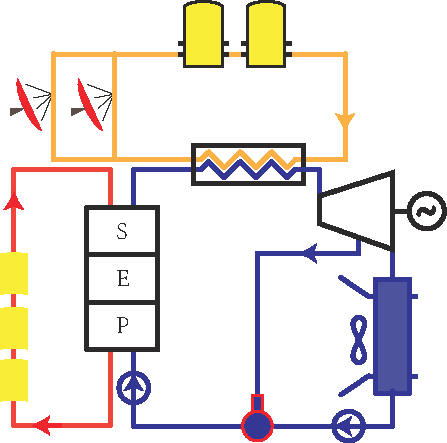
\includegraphics[width = \columnwidth]{fig/air-water1}
	\caption{}\label{fig:air-water_1}
	\end{subfigure}
	~
\begin{subfigure}[b]{0.4\columnwidth}
	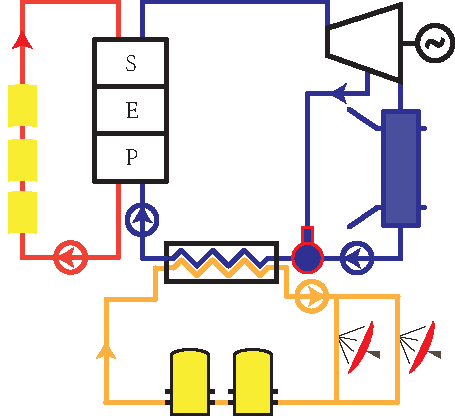
\includegraphics[width = \columnwidth]{fig/air-water2}
	\caption{}\label{fig:air-water_2}
	\end{subfigure}
	\caption{Schematic diagrams of two kinds of solar systems using air-water heat exchanger}
	\label{fig:air-water}
\end{figure}

%\begin{figure}[h]
%\centering 
%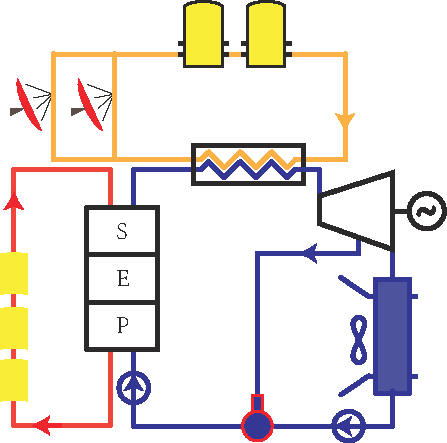
\includegraphics[width=0.6\textwidth]{fig/air-water1}
%\caption{schematic diagram of a solar system using air-water heat exchanger}\label{fig:air-water1}
%\end{figure}
%
%\begin{figure}[h]
%\centering 
%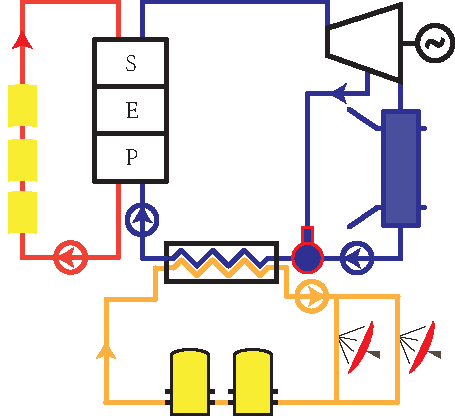
\includegraphics[width=0.6\textwidth]{fig/air-water2}
%\caption{schematic diagram of a solar system using air-water heat exchanger}\label{fig:air-water1}
%\end{figure}
\subsection{Heat recovery between cycles}
\label{sec:HRBC}

According to the second law of thermodynamics, it is impossible for any device that operates on a cycle to receive heat from a single reservoir and produces a net amount of work. For a heat engine, it requires both a hot source and a cold sink to convert heat energy to mechanical energy. 
Figure~\ref{fig:engines} shows the diagram of a typical heat engine. In a thermodynamic cycle, heat is absorbed from the hot source, only part of it can be converted into mechanical work by the engine. The conversion ratio related to the temperatures of hot source and cold sink is fundamentally limited by Carnot's theorem.

\begin{figure}[h]
\centering 
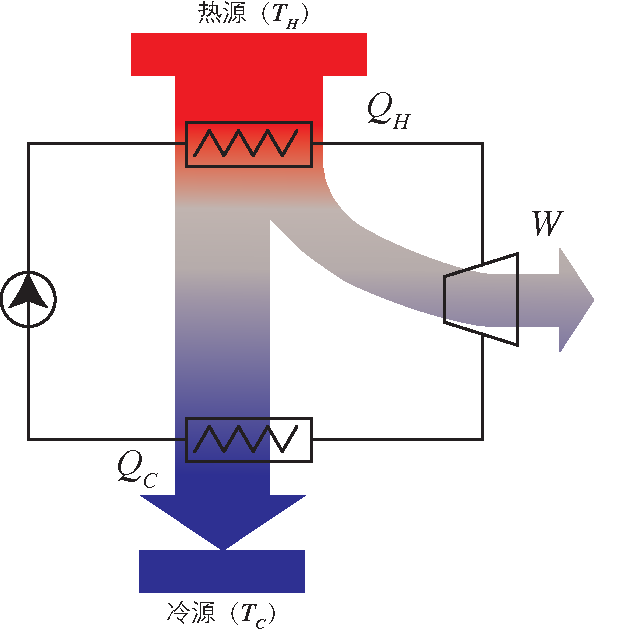
\includegraphics[width=0.5\textwidth]{fig/engines}
\caption{Diagram of a typical heat engine}\label{fig:engines}
\end{figure}

Only those engines suitable for external heating are usually considered for solar applications. Unlike an internal combustion engine that generates heat within the working fluid, an externally heated engine needs external heat to be added to the working fluid by a heat exchanger.

Three types of engines are designed to accept external heat and have been used for solar heat sources: the Rankine, the Stirling, and the Brayton cycles~\cite{Roschke1979}. The Rankine and Brayton cycles are both suitable for constant-pressure heat-addition. 
The original Brayton engine uses piston compressors and piston expanders, but more modern gas turbines and airbreathing jet engines also follow the Brayton cycle. Although the cycle is usually an open system, in order to carry out thermodynamic analysis, usually it is assumed that exhaust gases are reused as the intake so that the whole process can be analyzed as a closed cycle.
The Stirling machine uses a reciprocating piston design that allows external heating to be combined into its constant-temperature heat-addition process. 
In a Rankine cycle, the pressurized liquid enters a heat exchanger where it is heated at constant pressure by an external heat source to become vapor.

These three kinds of cycles work at different optimum operating temperatures. Rankine cycle works with the lowest hot source temperature and Brayton works with the highest. Figure~\ref{fig:cycles} shows the diagram of the three cycles used in solar energy. The heat released by these cycles may be recovered by another cycle (as a bottom cycle).

\begin{figure}[h]
\centering 
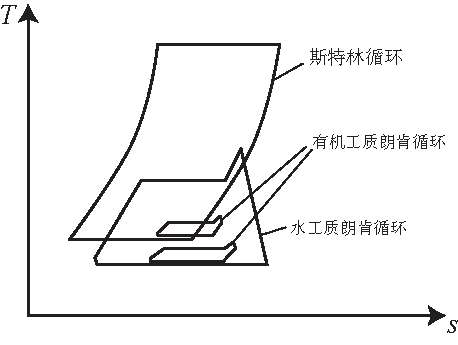
\includegraphics[width=0.5\textwidth]{fig/cycles}
\caption{Diagram of three cycles used in solar energy}\label{fig:cycles}
\end{figure}

\section{System topology selection}
\label{sec:sts}
\subsection{Rankine cycle fluid}

There are two important aspects to consider when selecting the working fluid of the Rankine cycle solar power system:
\begin{enumerate}
  \item Select the working fluid that is conducive to the optimization of the cycle efficiency.  
  For a Rankine cycle solar system, the collector efficiency reduces with operating temperature, and the Rankine cycle efficiency increases with operating temperature, there exists an optimal operating temperature as illustrated in Figure~\ref{fig:Efficiency}. The working fluid should be conducive to achieve the optimal operating temperature.
  
  \item The working fluid state matches the heat transfer fluid state, if heat transfer fluid is used.
    On the one hand, the operating temperature o78f the working fluid should be lower than the collecting temperature of the HTF. On the other hand, the operating temperature of the working fluid should not be much lower than the collecting temperature of the HTF to avoid large exergy loss during the heat exchange process.
\end{enumerate}
\begin{figure}[!ht]
\centering 
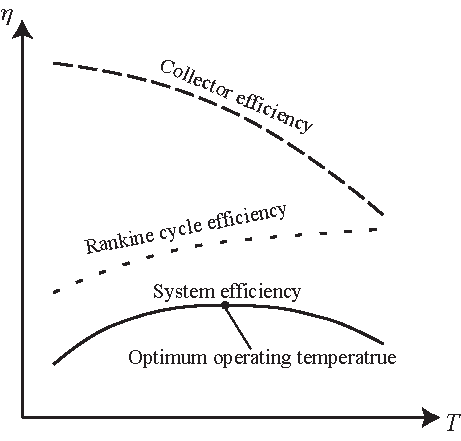
\includegraphics[width=0.5\textwidth]{fig/Efficiency}
\caption{Efficiency variation with operating temperature}\label{fig:Efficiency}
\end{figure}

Based on the advantages and disadvantages of water and organic fluid as the working fluid of Rankine cycle, it is clear that, for low operating temperature and small capacity distribution power generation, organic fluid will be a better choice, otherwise water is the better one. Bao and Zhao~\cite{Bao2013} presented a comprehensive review of working fluid selection (including pure fluids and mixtures). In this review, many factors such as operating conditions, working fluid characteristics, equipment structures and environmental safety considerations were considered.
It has to be mentioned that the types of working fluids (mainly dry or wet) will affect the operation and layout of the system.

\subsection{Solar chimney}

Section~\ref{sec:sc} shows the idea of coupling solar chimney to concentrated solar thermal power generation technologies.
However, the efficiency of current solar chimney system is still very low. Primary design data of solar chimney power plants with different location, different chimney height and collector height are shown in Table~\ref{tab:sc}~\cite{Bilgen2005}. The preliminary design parameters in Table~\ref{tab:sc} are selected and determined for a nominal solar intensity of 1000$\,\mathrm{W/m^2}$ and the nominal plant power of 5$\,\mathrm{MW}$. From the table, it can be found that the chimney efficiency and total efficiency are very low and the technology is still in the development stage.
\begin{table}[htbp]
	\caption{Results of SEA models under specified parameters}
	\begin{center}
	\begin{tabular}{ccccc}
		\toprule
		&Ottawa    &Winnipeg    &Edmonton    &Schlaich\\
		\midrule
		Collector diameter (m)    &	1110	&	1110	&	1110	&	1110 \\
  Collector area ($\mathrm{m^2}$)    & 950000    & 950000	&	950000	&	950000\\
  Chimney height (m)    &123    &60    &    35&    547\\
  Collector height (m)    &848    &975    &1024    &    -\\
  Chimney diameter (m)    &54    &54    &54    &54\\
  Temperature rise in collector ($\mathrm{^\circ C}$)    &25.9    &25.9    &25.9    &25.9\\
  Updraft velocity (m/s)&9.1    &9.1    &9.1    &9.1\\
  Total pressure head (Pa)&518.3    &518.3    &518.3    &383.3\\
  Average efficiency\\
  Collector (\%)    &56.00    &56.00    &56.00    &56.24\\
  Chimney (\%)    &1.82    &1.82    &1.82    &1.45\\
  Turbine (\%)    &77.0    &77.0    &77.0    &77.0\\
  Whole system (\%)    &0.79    &0.79    &0.79    &0.63\\
		\bottomrule
	\end{tabular}
	\end{center}
	\label{tab:sc}
\end{table}

%Besides, it will cost much more to apply a chimney tower in the demonstration system of this project. 
Besides, a solar chimney is costly and requires vast land, which is adverse to the future deployment of solar cascade demo system. With these considerations, the solar chimney plans are not adopted for the cascade system. 

\subsection{Collector series connection}
Each type of collector has its own suitable temperature range. It is feasible to heat the HTF step by step using different types of collectors with series connection.

A collector series connection is proposed in Section~\ref{sec:csc} (see Figure~\ref{fig:SeriesCollector}) depending on the basic systems. In this configuration, air is heated in the trough collectors and dish receivers consequently. After providing heat for the Stirling engines, the hot air flows into the heat exchanger to provide heat for the Rankine cycle. In this topology, air is used as the HTF for the solar trough, this idea is only numerically and experimentally studied,~\cite{Good2015,Good2016} no commercial applications can be found up to now. This technology is mainly constrained by the low conductivity and low heat capacity of air, which lead to low system efficiency. For this consideration, this topology is not adopted due to the parabolic trough collectors.

It can be a good choice to apply flat plate solar collectors and parabolic trough collectors in traditional solar tower power plant that uses water as the HTF (such as Solar One). As demonstrated in Figure~\ref{fig:seriesCollection}, condensed water is heated by the flat plate solar collectors and feedwater is heated by the parabolic trough collectors. Flat plate collectors and parabolic trough collectors have much lower unit thermal cost compared to solar tower. The addition of flat plate collectors and parabolic trough collectors can effectively reduce the cost of the system. Although this scheme is promising and deserves further research, the cascade system in this thesis will not consider it for the requirement of solar tower is adverse to the deployment of cascade demo system.

\begin{figure}[!ht]
\centering 
\includegraphics[width=0.5\textwidth]{fig/SeriesCollection}
\caption{Schematic diagram of a cascade system using collector series connection}\label{fig:seriesCollection}
\end{figure}

\subsection{Direct steam generation}
Direct steam generation for solar thermal power generation has the advantage of having fewer components and no temperature drop due to an intermediate transfer. Besides, it is clear that water is characterized by lower environmental risk than thermal oil so that leakages in a DSG power plant do not represent an environmental hazard ~\cite{Fernandez2010}. Water has a lower freezing temperature than thermal oil and above all than solar salt: the efforts required to ensure adequate anti-freezing protection are significantly reduced. Water is also less corrosive than solar salt~\cite{Giglio2017}. With both liquid and vapor in a receiver, however, extreme care must be taken in the design of the receiver to ensure that the radiant flux incident on that portion of the receiver containing vapor is less than the flux incident in the regions with liquid and where boiling is taking place. This is because the heat-transfer coefficient into a liquid is significantly higher than into superheated vapor. For similar values of solar flux, burnout of the receiver walls could occur in the regions where vapor exists on the other side of the receiver wall.

Many concentrating collector designs require that the receiver change attitude while the collector tracks the sun. This change of attitude increases the chances of high flux on portions of the receiver containing vapor.
Two examples of solar Rankine power systems where the engine working fluid vapor is generated directly in the receiver are the Solar One Pilot Plant at Barstow, CA and the solar organic Rankine cycle module built by Ford Aerospace and Communications Corporation. Because Solar One is a central receiver system, the vertical-tube receiver remains stationary and liquid level control is relatively easy. The vertical tubes of the receiver are made of a material with a high melting point and thus can withstand high temperatures in the upper regions where vapor is being superheated. Tube burnout is avoided in the Ford Aerospace receiver design because the inner wall of the receiver is a copper shell with tubes wound around its exterior. The high thermal conductivity of the copper shell provides an averaging effect on receiver temperature, and superheat is attained without burnout of the receiver walls.

All the CSP commercial plants already built apply indirect steam generation, with the exception of the 5 MWe DSG Thai Solar One (TSE-1) plant in Thailand (Thailand, 2012)~\cite{Khenissi2015}. The reason for this universally accepted choice must be found in the difficulties related to the flow control and manufacturing of equipment to be used in the presence of a two-phase flow in the absorber tubes. The behavior of the two-phase flow inside the absorber tubes of a parabolic-trough collector forces the implementation of a complex and expensive control system and the use of fast water streams in order to avoid stratified flow.
			
Another problem related to the DSG is the high value of the steam pressure inside the receiver tubes that must match the turbine inlet pressure for less than pressure losses. Indeed, handling the moveable and flexible components forming the receiver tube of the collector in case of high-pressure values was one of the main problems to be faced at the early stages of the DSG concept technology. 

Apply direct steam generation may be a better choice in the cascade system, however, it is not adopted for the cascade system for its immaturity.

\subsection{Heat exchanger between circuits}

Section~\ref{sec:hebc} introduces two types of heat exchangers that may be applied in the solar thermal cascade system -- the air-oil heat exchanger (see in Figure~\ref{fig:air-oil_c}) and the air-water heat exchanger (see in Figure~\ref{fig:air-water_c}). 

\begin{figure}[h]
\centering 
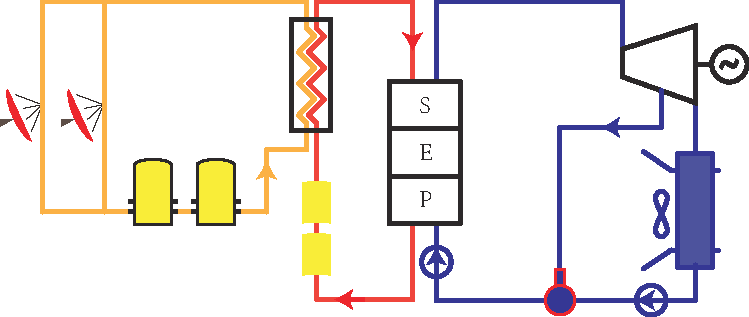
\includegraphics[width=0.7\textwidth]{fig/air-oil}
\caption{Schematic diagram of a solar system using air-oil heat exchanger}\label{fig:air-oil_c}
\end{figure}

\noindent \begin{figure}[htbp]
\centering
	\begin{subfigure}[b]{0.4\columnwidth}
	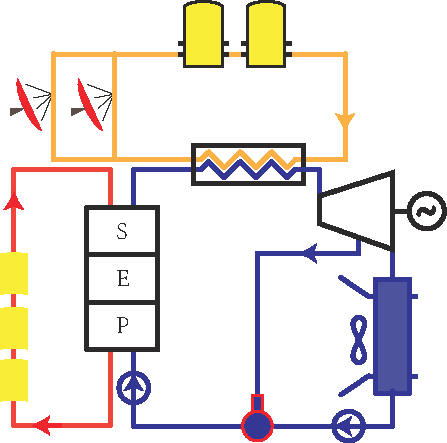
\includegraphics[width = \columnwidth]{fig/air-water1}
	\caption{}\label{fig:air-water_1_c}
	\end{subfigure}
	~
\begin{subfigure}[b]{0.4\columnwidth}
	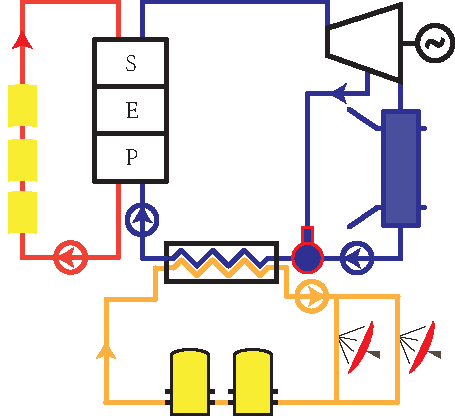
\includegraphics[width = \columnwidth]{fig/air-water2}
	\caption{}\label{fig:air-water_2_c}
	\end{subfigure}
	\caption{Schematic diagrams of two kinds of solar systems using air-water heat exchanger}
	\label{fig:air-water_c}
\end{figure}

For the first type, air provides heat for oil. It is not economic for several reasons. First, The temperature of the heat transfer oil can not be further increased. The temperature of the oil is not limited by the parabolic trough collectors. The temperature of the oil is constrained by the oil properties and heat collecting temperature of the trough collectors can exceed this value. In high temperature conditions, oil may deterioration, evaporation, decompose, which has a negative impact on the stable and safe operation of the system. Second, using dish to provide heat for the oil is not suitable since the dish is designed for higher temperature collections and it's less cost-effective compared with parabolic trough.

For the second type, air provides heat for water. Two kinds of solar systems using air-water heat exchanger can be found in Figure~\ref{fig:air-water_c}. Figure~\ref{fig:air-water_1_c} shows the scheme that air after the Stirling engine is used to overheat the steam. It's feasible since the air can increase the average temperature of the endothermic process of the water to increase the efficiency of Rankine cycle. On the other hand, in the traditional solar trough system, the main steam temperature is limited by the oil, which is not conductive to Rankine cycle efficiency. In this proposed cascade system, the main steam temperature of the Rankine cycle can be raised to be higher than 400$\mathrm{^\circ C}$ to eliminate the negative effect of the oil.
This is the scheme that will be discussed in detail in the next few chapters. Figure~\ref{fig:air-water_2_c} shows the scheme that air after the Stirling engine is used to preheat the feed water. It is not a good choice since the temperature difference of the heat transfer process is large and it provides no benefits to increase the inlet temperature of the steam turbine.
 
\subsection{Heat recovery between cycles}
As it is mentioned in Section~\ref{sec:HRBC}, different thermodynamic cycles work at different optimum working temperatures. Since each thermodynamic cycle has endothermic and exothermic processes, a bottoming cycle may use the released heat of a topping cycle.

\noindent \begin{figure}[htbp]
\centering
	\begin{subfigure}[b]{0.4\columnwidth}
	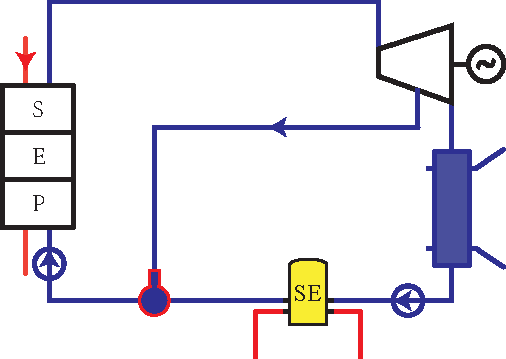
\includegraphics[width = \columnwidth]{fig/Stirling-Rankine}
	\caption{}\label{fig:Stirling-Rankine}
	\end{subfigure}
	~
\begin{subfigure}[b]{0.4\columnwidth}
	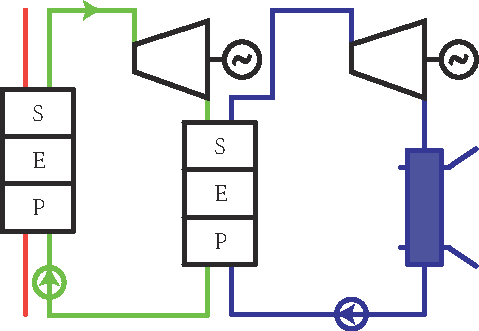
\includegraphics[width = \columnwidth]{fig/SeriesRankine}
	\caption{}\label{fig:Rankine-Rankine}
	\end{subfigure}
	\caption{Two configurations with heat recovery between thermodynamic cycles}
	\label{fig:coupledCycles}
\end{figure}

In our basic systems (see Figure~\ref{fig:PTPD}), Rankine cycle and Stirling cycle can be coupled for cascade usage. 
Figure~\ref{fig:coupledCycles} shows two configurations of the cascade systems with heat recovery between cycles. 
For a traditional Stirling engine, to enhance the performance, cooling water is used to absorb the heat released by the engine. The absorbed heat is wasted without reuse.
In Figure~\ref{fig:Stirling-Rankine}, condensate of the Rankine cycle is used to cool the Stirling engine. Rejected heat of the Stirling cycle can be reused by Rankine cycle. 
For organic Rankine cycles, different working fluids determine the working temperature zones. It is feasible to reuse the condensation heat of an organic Rankine cycle by another organic Rankine cycle.
In Figure~\ref{fig:Rankine-Rankine}, two organic Rankine are coupled together for power generation. The bottoming cycle uses the condensation heat of the topping cycle for preheating, evaporation and superheating.
%补充

\section{Selected system topology}
\label{sec:sst}
Considered all the conditions in Section~\ref{sec:std} and Section~\ref{sec:sts}, two system topologies are chosen for this research as shown in Figure~\ref{fig:CascadeSystems}. 

%第二种方案需要考虑是否用两个空气换热器
\noindent \begin{figure}[htbp]
\centering
	\begin{subfigure}[b]{0.4\columnwidth}
	\includegraphics[width = \columnwidth]{fig/CascadeSystem1}
	\caption{}\label{fig:CascadeSystem1}
	\end{subfigure}
	~
\begin{subfigure}[b]{0.4\columnwidth}
	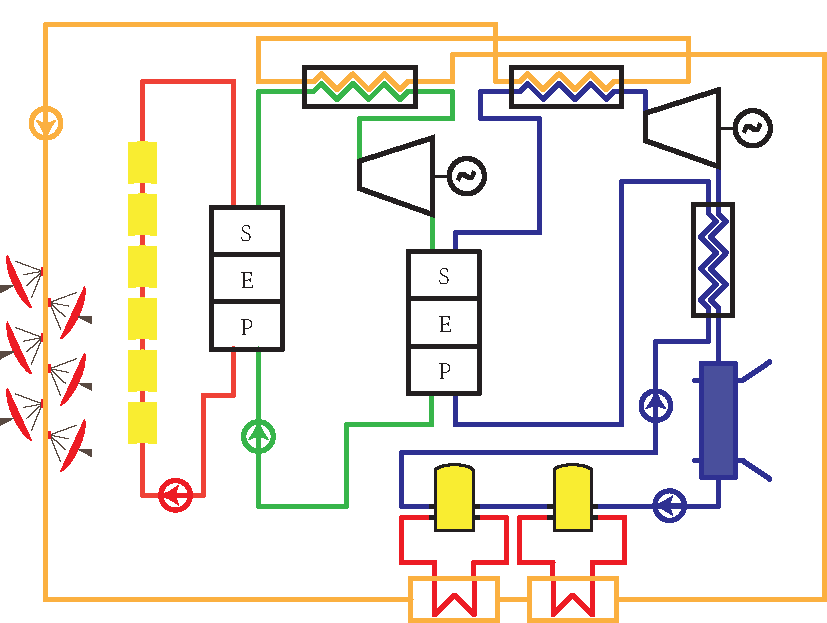
\includegraphics[width = \columnwidth]{fig/CascadeSystem2}
	\caption{}\label{fig:CascadeSystem2}
	\end{subfigure}
	\caption{Two selected typical cascade system}
	\label{fig:CascadeSystems}
\end{figure}

In Figure~\ref{fig:CascadeSystem1}, the cascade system has the following features:

\begin{itemize}
  \item \emph{Multiple types of collectors.} Trough collectors are applied for lower temperature heat collection and Dish collectors are applied for higher temperature heat collection. This helps to reduce the cost and improve the efficiency.
  \item \emph{Multiple types of thermodynamic cycles.} Rankine cycle is applied for lower temperature heat utilization. Stirling cycle is applied for higher temperature heat utilization.
  \item \emph{Air-water heat exchanger.} An extra air-water heat exchanger is applied to increase the temperature of the main steam, which helps to improve the efficiency of Rankine cycle. On the other hand, it can overcome the disadvantage of low limit temperature of heat transfer oil in traditional solar trough systems, which helps to achieve higher main steam parameters than traditional solar trough systems. 
  \item \emph{Condensate for Stirling engine cooling.} Condensate of the Rankine cycle is used to cool the Stirling engine. Rejected heat of the Stirling cycle can be reused by Rankine cycle, which helps to improve the overall system efficiency.
\end{itemize}

In Figure~\ref{fig:CascadeSystem2}, the cascade system also has the features mentioned above. Besides, it uses different kinds of organic fluid as the working fluid, which adapts more general working temperature for solar energy systems. Figure~\ref{fig:Ex_CascadeSystem2} shows a calculation example of the cascade system.

\begin{figure}[!ht]
\centering 
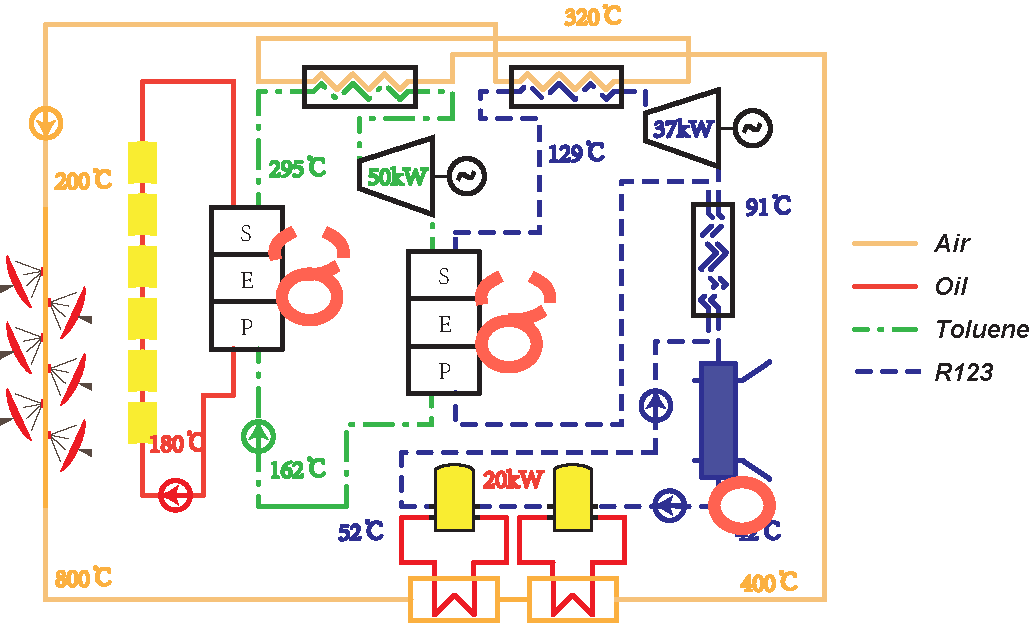
\includegraphics[width=0.7\textwidth]{fig/Ex_CascadeSystem2}
\caption{A calculation example of cascade system in Figure~\ref{fig:CascadeSystem2}}
\label{fig:Ex_CascadeSystem2}
\end{figure}

Both cascade systems will be modeled for investigation. However, considering the more extensive application of the steam Rankine cycle, the system as described in Figure~\ref{fig:CascadeSystem1} will be used as the main research content in the following chapters.

\section{Conclusion}
This chapter systematically introduces a number of considerations in cascade solar thermal system design. These considerations include Rankine cycle fluid type, solar chimney, collector series connection, direct steam generation, heat exchanger between circuits and heat recovery between cycles. 

These considerations are carefully checked for the cascade system study. Combining with the research direction, two typical system topologies suitable for the deployment of cascade demo system are put forward. These two typical system topologies have the following features:

\begin{itemize}
  \item Multiple types of collectors are applied.
  \item Multiple types of thermodynamic cycles are applied. 
  \item Air-water heat exchanger is applied to increase the Rankine cycle efficiency.
  \item Condensate for Stirling engine cooling to recover the heat rejected by the engine.
\end{itemize}

It is worthy noting that some of the considerations of the system topology design deserves more concern in the future. For example, a solar power tower combined with parabolic trough collectors and flat plates as shown in Figure~\ref{fig:seriesCollection} effectively utilizes the characteristics of the collectors. When the technology of direct steam generation is mature, it is worthy to apply it in cascade system for its less equipment required and no temperature loss feature.